% !TEX TS-program = arara
% arara: xelatex: { synctex: on, options: [-halt-on-error] } 
% arara: biber
%% arara: makeglossaries
%% arara: makeindex
% arara: xelatex: { synctex: on, options: [-halt-on-error] } 
% arara: xelatex: { synctex: on, options: [-halt-on-error]  } 
% arara: clean: { extensions: [ aux, log, out, run.xml, toc, mw, synctex.gz, ] }
% arara: clean: { extensions: [ bbl, bcf, blg, ] }
%% arara: clean: { extensions: [ glg, glo, gls, ] }
% arara: clean: { extensions: [ idx, ] }
%% arara: clean: { extensions: [ ilg, ind, xdy, ] }
%% arara: clean: { extensions: [ plCode, plData, plMath, plExercise, plNote, plQuote, ] }
%-----------------------------------------------------------------
\documentclass{PalisadesLakesArticle}
%-----------------------------------------------------------------
%Note:  requires bib directory defined in arara call to biblatex
\addbibresource{algebra.bib}
\addbibresource{arithmetic.bib}
\addbibresource{cactus.bib}
\addbibresource{feferman.bib}
\addbibresource{halmos.bib}
%\addbibresource{ieeestd.bib}
\addbibresource{interpolation.bib}
\addbibresource{logic.bib}
\addbibresource{math.bib}
\addbibresource{mcdonald.bib}
\addbibresource{mop.bib}
\addbibresource{numbers.bib}
\addbibresource{proglang.bib}
\addbibresource{sets.bib}
\addbibresource{tex.bib}
\addbibresource{topos.bib}
%-----------------------------------------------------------------

\geomAfour
\geomPortraitTwoColumn
%-----------------------------------------------------------------
\title{Article template}
\author{John Alan McDonald 
(palisades dot lakes at gmail dot com)}
\date{draft of \today}
%-----------------------------------------------------------------
\begin{document}
\maketitle
\PalisadesLakesTableOfContents
%-----------------------------------------------------------------

\begin{plQuote}
{\citeAuthorYearTitle{Thurston:1994:Proof}}{}%
{Mathematics as we practice it is much more formally 
complete and precise than
other sciences, but it is much less formally complete and precise 
for its content than computer programs.
}
\end{plQuote}

\begin{plSection}{Colors}

\begin{plPlot}{}{}{}
\end{plPlot}
\begin{plTable}{}{}{}
\end{plTable}
\begin{plQuote}{}{}{}
\end{plQuote}
\begin{plAlgorithm}{}{}{}
\end{plAlgorithm}
\begin{plListing}{}{}{}
\end{plListing}
\begin{plScreen}{}{}{}
\end{plScreen}

\begin{plNote}{}{}{}
\end{plNote}

\begin{plExercise}{}{}{}
\end{plExercise}

\begin{plDefinition}{}{}{}
\end{plDefinition}
\begin{plExample}{}{}{}
\end{plExample}
\begin{plAxiom}{}{}{}
\end{plAxiom}
\begin{plAxiomSchema}{}{}{}
\end{plAxiomSchema}
\begin{plLemma}{}{}{}
\end{plLemma}
\begin{plTheorem}{}{}{}
\end{plTheorem}
\begin{plCorollary}{}{}{}
\end{plCorollary}
\begin{plDiagram}{}{}{}
\end{plDiagram}

\end{plSection}%{Colors}
%-----------------------------------------------------------------
\def\sharedFolder{../shared/}
\import{\sharedFolder}{writing}
%-----------------------------------------------------------------
\import{\sharedFolder}{computation}
%-----------------------------------------------------------------
\import{\sharedFolder}{mathematics}
%-----------------------------------------------------------------
\begin{plSection}{Applications}
\begin{plSection}{Geometry}
\end{plSection}%{Geometry}
\begin{plSection}{Layout}
\end{plSection}%{Layout}
\begin{plSection}{Design}
\end{plSection}%{Design}
\begin{plSection}{Visualization}
\end{plSection}%{Visualization}
\begin{plSection}{Cartography}
\end{plSection}%{Cartography}
\begin{plSection}{Prediction}
\end{plSection}%{Prediction}
\begin{plSection}{Planning}
\end{plSection}%{Planning}
\begin{plSection}{Control}
\end{plSection}%{Control}
\begin{plSection}{Fonts}
\end{plSection}%{Fonts}
\begin{plSection}{Vision}
%-----------------------------------------------------------------
\begin{plSection}{Removing diffraction blur}
\end{plSection}%{Removing diffraction blur}
%-----------------------------------------------------------------
\end{plSection}%{Vision}
\begin{plSection}{Sound}
\end{plSection}%{Sound}
%-----------------------------------------------------------------
\begin{plSection}{Curves and Surfaces}
%-----------------------------------------------------------------
\import{\sharedFolder}{simplicial-meshes}
\import{\sharedFolder}{barycentric-coordinates}
\import{\sharedFolder}{volume}
\import{\sharedFolder}{mesh-operations}
\import{\sharedFolder}{flatten}
%-----------------------------------------------------------------
\import{\sharedFolder}{interpolation}
%-----------------------------------------------------------------
\import{\sharedFolder}{curves}
%-----------------------------------------------------------------
\begin{plSection}{Triangular Meshes}
\import{\sharedFolder}{faces}
\import{\sharedFolder}{edges}
\import{\sharedFolder}{vertices}
\end{plSection}%{Triangular Meshes}}
%-----------------------------------------------------------------
\import{\sharedFolder}{subdivision}
%-----------------------------------------------------------------
\begin{plSection}{Fitting}
\import{\sharedFolder}{data-fitting}
\import{\sharedFolder}{image-fitting}
\import{\sharedFolder}{registration}
\import{\sharedFolder}{averaging}
\end{plSection} % Fitting
%-----------------------------------------------------------------
\end{plSection}%{Curves and Surfaces}
%-----------------------------------------------------------------
\end{plSection}%{Applications}
%-----------------------------------------------------------------
\BeginAppendices
%-----------------------------------------------------------------
\begin{plSection}{Typesetting}

This document was typeset using Mik\TeX{} $2.9$ \cite{Schenk:2017:Miktex} 
and {\TeX}works $0.6.5$ \cite{KewLoffler:2017:Texworks} 
on \textsc{Windows} $10$. 
I used \texttt{arara} \cite{CeredaEtAl:2021:Arara} 
to run \texttt{xelatex}, \texttt{biber}, \texttt{makeglossaries},  and
\texttt{texindy: { markup: xelatex }}.
I believe only Mik\TeX\  and {\TeX}works are Windows specific; 
the actual typesetting tools should be usable on Linux and MacOS as well.

See also \cite{Talbot:2012:LatexNovices,Talbot:2013:LatexPhD}.

\begin{plScreen}
{Configuring {\TeX}works for \texttt{arara}.}
{fig:arara}
\centering
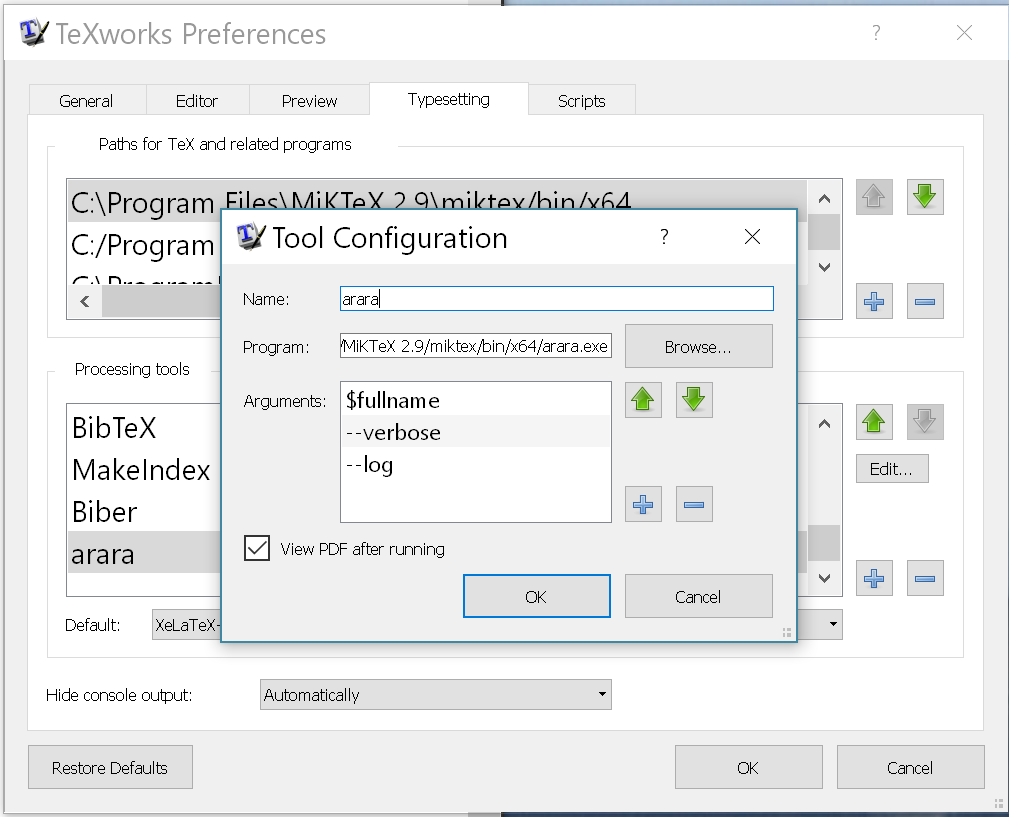
\includegraphics[scale=0.75]{../figs/arara.png}
\end{plScreen}
\vfill
\end{plSection}%{Typesetting}

%-----------------------------------------------------------------

\end{document}
%-----------------------------------------------------------------
